\chapter{Prestazioni}
\label{prestazioni}

In questo capitolo si mostra l'esito in termini di performance delle modifiche apportate. Le prestazioni sono state misurate tramite uno script ereditato dal lavoro precedente sulla libreria FIDO opportunamente modificato per lo scopo. 

\section{Raccolta dei dati}
\label{raccolta_dati}

Per prendere le misurazioni relative alle performance è stato utilizzato un calcolatore con sistema operativo Fedora 36, dotato di CPU Intel i5-8250U e un autenticatore CTAP2 emulato virtualmente tramite il backend UDP descritto nel capitolo precedente \ref{testing}. Grazie all'emulatore è stato possibile inibire la mediazione dell'utente richiesta, in fase sia di creazione delle credenziali che di autenticazione. In tal modo, il dato ottenuto risulta deterministico.

I tempi di esecuzione sono stati presi tramite l'ausilio della libreria Python \verb*|timeit|, che include metodi per la misura del tempo di esecuzione di funzioni. Tali metodi accettano come parametri la funzione da misurare e il numero di volte che deve essere eseguita, restituendone il tempo di esecuzione. I metodi misurati sono quelli descritti nei capitoli precedenti:

Per la fase di creazione delle credenziali
\begin{itemize}
	\item \verb*|register_begin()|
	\item \verb*|make_credential()|
	\item \verb*|register_complete()|
\end{itemize}
E per la fase di autenticazione
\begin{itemize}
	\item \verb*|authenticate_begin()|
	\item \verb*|get_assertion()|
	\item \verb*|authenticate_complete()|
\end{itemize}

Per ogni livello di sicurezza $|Q|$ stabilito, il numero $n$ di server presenti e il numero \emph{k} di server malevoli con $k \in [1,n]$, i test sono stati ripetuti con un livello di sicurezza $|Q| \in [2k+1, 3k+1]$. Per diminuire la variabilità dei dati i tempi del metodo \verb*|get_assertion()| sono stati presi sulla base della media di dieci iterazioni. La fase di creazione è stata, invece, ripetuta solamente una volta.

\section{Valutazione dei dati}
\label{valutazione}

I dati nel grafico sono relativi alle fasi sia di creazione che di autenticazione, cioè al tempo totale misurato.
\begin{center}
	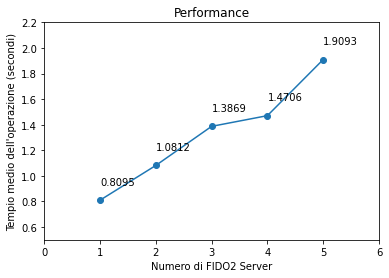
\includegraphics[scale=0.65]{figures/test_results}
\end{center}

Come si può notare dal grafico all'aumentare del numero di FIDO Server l'operazione totale subisce un incremento di circa 20 \emph{ms}. 

I tempi per la fase di registrazione riportano un risultato simile: un incremento di circa 13 \emph{ms} ogni tre FIDO Server aggiuntivi.
\begin{center}
	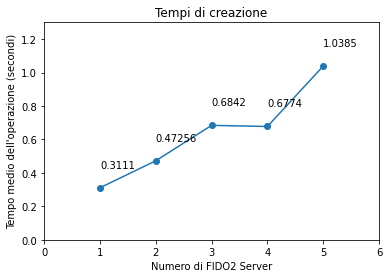
\includegraphics[scale=0.65]{figures/creation_results}
\end{center}

Nella figura successiva sono rappresentati i tempi misurati per la sola fase di autenticazione. Per ogni valore di \emph{k} sono stati utilizzati i valori di security level nel range $[2k+1, 3k+1]$. Come si può notare la variazione del livello di sicurezza, dato lo stesso numero di server malevoli tollerabili, non influenza sensibilmente i tempi dell'operazione.
\begin{center}
	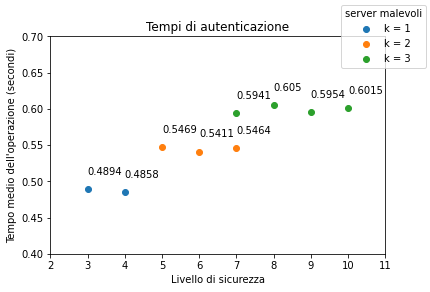
\includegraphics[scale=0.65]{figures/auth_results}
\end{center}

Occorre precisare che le misurazioni effettuate sono assolutamente ottimistiche per quanto riguarda la latenza sia con i FIDO Server, operanti localmente, sia con l'autenticatore, emulato virtualmente. Inoltre, non tengono conto dell'interazione umana richiesta e dell'utilizzo di un Web Browser con le penalizzazioni che ne conseguono. 

Si può quindi concludere dai dati raccolti che l'incremento di tempo richiesto dall'operazione con una combinazione di $|Q|$ e \emph{n} è di pochi \emph{ms} in più a fronte di una \emph{survivability} migliore. La parte più onerosa in termini di tempo è quella legata alla registrazione, la quale richiede il doppio del tempo al raddoppiare dei FIDO Server con cui dialogare. La fase di autenticazione, invece, si distanzia di soli $12 ms$ tra il caso limite inferiore e quello superiore considerato, con un incremento pari circa al $25\%$.

\section{Fattibilità}
\label{fattibilità}

Come specificato nella sezione relativa ai dettagli implementativi \ref{testing}, è stato utilizzato un emulatore dell'autenticatore hardware sviluppato da Solokeys sia per l'implementazione che per la fase di testing. Il codice dell'autenticatore originale è basato sul microcontrollore STM32L432, che offre 256KB di memoria secondaria. L'implementazione suddivide la memoria secondaria nel seguente modo:
\begin{itemize}
	\item 14 KB per il bootloader
	\item 226 KB per il codice da eseguire
	\item 16 KB disponibili per immagazzinare i dati, di cui solo 2048 B adibite alla memorizzazione del contatore
\end{itemize}

Poiché la memoria disponibile è così ridotta gli sviluppatori hanno previsto il cosidetto \emph{wrapping delle chiavi}: piuttosto che generare una coppia di chiavi crittografiche ad ogni richiesta di registrazione, viene generata una singola chiave crittografica \textbf{M} detta \emph{master key} e ad ogni richiesta di registrazione viene computato l'hash di \emph{HMAC(R, M)} dove \textbf{R} è un numero generato al momento. Il risultato dell'hash è una chiave crittografica, da cui verrà derivata la corrispondente chiave pubblica. La prima viene usata per firmare e la seconda viene inviata al server insieme ad \textbf{R}. Nessuna informazione viene salvata dall'autenticatore: l'unico dato necessario all'autenticatore in fase di autenticazione è \textbf{R}, tramite il quale ripeterà il procedimento computando l'\emph{hash} per generare le chiavi. 

Dato che l'implementazione proposta si avvale di una struttura dati \verb*|signCounter| che presenta:
\begin{itemize}
	\item Una struttura dati CredentialID di dimensioni pari a $88$ bytes
	\item Un array di contatori interi senza segno di 16 bit l'uno, i quali garantiscono 1 autenticazione al giorno per 179 anni ($(2^{16}) \div 365$), per 3 livelli di sicurezza
\end{itemize}


Avremo quindi una occupazione di memoria del \verb*|signCounter| di circa $94$ bytes. Per rispettare i vincoli di memoria dell'autenticatore, nella soluzione proposta, come nel firmware dell'autenticatore originale, dedichiamo 2048 bytes alla memorizzazione dei contatori. In questo modo è possibile immagazzinare circa \textbf{21} credenziali differenti. Il risultato ottenuto è in linea con i limiti stabiliti \cite{yubico:resident} da Yubico per le proprie \emph{resident keys}, una tipologia particolare di credenziali che necessitano di essere salvate in memoria.

Occorre considerare che l'aggiunta di un contatore limita le possibilità dell'hardware, di fatto riducendo il rapporto costo microcontrollore/numero di credenziali. Si può stimare un costo a contatore ($21$ credenziali * $ 3$ livelli di sicurezza), con un prezzo dell'STM32L432 per grossi stock di $\$4.59673$, di circa $0,07$ cents, sicuramente non trascurabile per grandi numeri.

La potenzialità di utilizzare la chiavetta per autenticarsi a virtualmente un numero illimitato di servizi Web viene a mancare, ma ciò è compensato da livelli di sicurezza del tutto sufficienti a garantire un incremento di sicurezza notevole (si parla di una resistenza fino a due server compromessi) e un utilizzo giornaliero costante e duraturo. Considerando anche la limitatezza di servizi Web che offrono l'autenticazione passwordless, si può concludere che il limite di ventuno credenziali non è affatto stringente. 